\documentclass{standalone}

\usepackage{tikz}
\usetikzlibrary{calc}
\usetikzlibrary{math}


\def\memory#1#2#3#4{
  \begin{scope}
    \def\names{#2}
    \def\values{{#3}}

    \node at ($ #1 + (1, -0.2) $) {\tiny #4};
    \draw[fill=gray!10] #1 rectangle ++(2, 2.75);

    \foreach \name [count=\i] in \names
    {
      \tikzmath{\val= \values[\i-1];}

      \node at ($ #1 + (0.4, -0.5 + \i * 1.25) $) {\name};
      \draw[draw=black, fill=white] ($ #1 + (0.75, -1 + \i * 1.25) $) rectangle ++(1, 1)
                        node[pos=.5] {\val};
    }
  \end{scope}
}

\begin{document}
  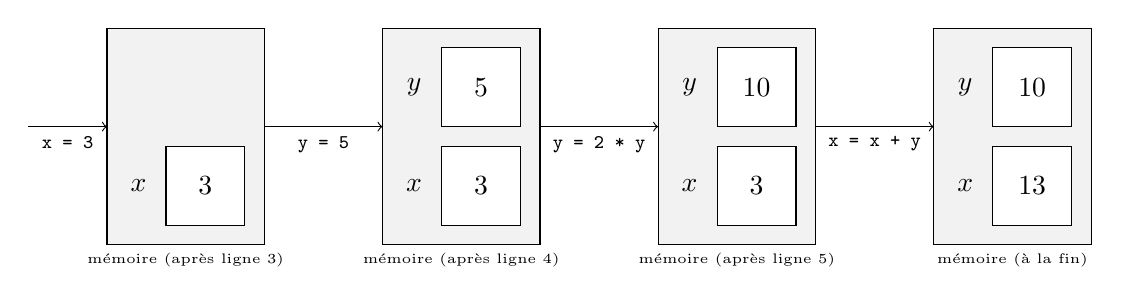
\begin{tikzpicture}
    \memory{(0, 0)}{$x$}{3}{m\'emoire (apr\`es ligne 3)}
    \memory{(3.5, 0)}{$x$, $y$}{3, 5}{m\'emoire (apr\`es ligne 4)}
    \memory{(7, 0)}{$x$, $y$}{3, 10}{m\'emoire (apr\`es ligne 5)}
    \memory{(10.5, 0)}{$x$, $y$}{13, 10}{m\'emoire (\`a la fin)}

    \draw[->] (-1, 1.5) -- node [below] {\scriptsize\texttt{x = 3}} (0, 1.5);
    \draw[->] (2, 1.5) -- node [below] {\scriptsize\texttt{y = 5}} (3.5, 1.5);
    \draw[->] (5.5, 1.5) -- node [below] {\scriptsize\texttt{y = 2 * y}} (7, 1.5);
    \draw[->] (9, 1.5) -- node [below] {\scriptsize\texttt{x = x + y}} (10.5, 1.5);
  \end{tikzpicture}
\end{document}
